\documentclass[10pt,twocolumn,letterpaper]{article}

% --- Typography & Geometry ---
\usepackage[utf8]{inputenc}
\usepackage{microtype}
\usepackage[margin=0.75in,top=0.85in,bottom=0.85in]{geometry}

% --- Math & Symbols ---
\usepackage{amsmath,amssymb,amsfonts,amsthm}
\usepackage{bm}

% --- Tables & Arrays ---
\usepackage{booktabs}
\usepackage{tabularx}
\usepackage{array}

% --- Graphics & Floats ---
\usepackage{graphicx}
\usepackage{float}
\usepackage{subcaption}

% --- Code Listings ---
\usepackage{xcolor}
\usepackage{listings}

\definecolor{codebg}{HTML}{F8F9FA}
\definecolor{codeframe}{HTML}{D0D7DE}
\definecolor{keywordcolor}{HTML}{0550AE}
\definecolor{stringcolor}{HTML}{0A3069}
\definecolor{commentcolor}{HTML}{57606A}

\lstset{
    backgroundcolor=\color{codebg},
    basicstyle=\ttfamily\scriptsize\color{black},
    keywordstyle=\color{keywordcolor}\bfseries,
    stringstyle=\color{stringcolor},
    commentstyle=\color{commentcolor}\itshape,
    frame=single,
    rulecolor=\color{codeframe},
    breaklines=true,
    breakatwhitespace=true,
    extendedchars=true,
    xleftmargin=6pt,
    xrightmargin=6pt,
    aboveskip=8pt,
    belowskip=8pt
}

% --- Hyperlinks ---
\usepackage{hyperref}
\hypersetup{
    colorlinks=true,
    linkcolor=blue!70!black,
    citecolor=blue!70!black,
    urlcolor=blue!70!black
}

% --- Input Title & Authors ---
% Metadata for orion
\title{\textbf{ORION: Optimized Rectified Input-aware Orthogonal Network for Hybrid Attention with SVD Factorization}}

\author{
  \textbf{Taha Majs}\thanks{Corresponding author: tahamajs@uni.edu} \quad \textbf{Research Team} \\
  Department of Computer Science \\
  Advanced Machine Learning \& Efficiency Laboratory
}

\date{\today}


\begin{document}

\maketitle

% --- Abstract & Keywords Block ---
\begin{abstract}

We present \textbf{ORION} (Optimized Rectified Input-aware Orthogonal Network), 
a hybrid attention mechanism that combines three orthogonal ideas: 
(i) \textbf{zero-shot SVD low-rank factorization} of Q/K/V/O projection weights, 
(ii) \textbf{head-wise bifurcation} between a linear-attention kernel branch 
(2/3 of heads) and a full softpick branch (1/3 of heads), and (iii) 
\textbf{random Fourier features} for the kernel heads. Unlike prior hybrid 
attention modules in our framework (e.g., NHA, NASC, GoldFinch), ORION 
\textbf{genuinely reduces parameter count}: each projection $W \in \mathbb{R}^{d_\text{out} \times d_\text{in}}$ 
is replaced by a product $W_\text{up} W_\text{down}$ with intermediate rank 
$r = 64$, achieving ~6$\times$ reduction for $768 \times 768$ projections and ~9.6$\times$ 
for $768 \times 3072$ FFN-like projections.

We evaluate ORION on DistilBERT, RoBERTa, and GPT-2 on SST-2 with LoRA 
recovery at rank $r_L = {{LORA_RANK}}$. ORION achieves \textbf{{{D\_ACC}}\%} on 
DistilBERT (baseline {{D\_BASE}}\%, $\Delta$ = {{D\_DELTA}}), \textbf{{{R\_ACC}}\%} on 
RoBERTa ($\Delta$ = {{R\_DELTA}}), and \textbf{{{G\_ACC}}\%} on GPT-2 ($\Delta$ = {{G\_DELTA}}). 
Parameter count decreases by \textbf{{{PARAM\_REDUCTION}}\%} across all models. 
We document one critical implementation bug: \texttt{copy\_weights} \textbf{raises} on 
UniversalAdapter failure instead of falling back, matching the pattern 
observed in other modules and causing catastrophic collapse when triggered.

\textbf{Keywords:} SVD factorization, hybrid attention, kernel attention, 
softpick, random Fourier features



\vspace{0.5em}
\noindent\textbf{Keywords:} SVD factorization, hybrid attention, kernel attention,
\end{abstract}

\vspace{1em}

% --- Paper Body ---
\section{01 Intro}

Draft content for orion.


\section{Related Work}

\subsection{Low-Rank Compression}

\textbf{SVD factorization} (Eckart \& Young, 1936). The optimal rank-$r$ 
approximation in Frobenius norm.

\textbf{ALBERT} (Lan et al., 2020). Cross-layer parameter sharing.

\textbf{Tensor train} (Novikov et al., 2015). Higher-order factorization.

\textbf{ORION uses SVD} with energy-based rank selection.

\subsection{Linear Attention}

\textbf{Linear Transformer} (Katharopoulos et al., 2020). $\phi(x) = \text{elu}(x) + 1$.

\textbf{Performer} (Choromanski et al., 2021). Random Fourier Features.

\textbf{Cosformer} (Qin et al., 2022). Cosine reweighting.

\textbf{ORION uses RFF} for the kernel heads.

\subsection{Hybrid Attention}

\textbf{Longformer} (Beltagy et al., 2020). Sliding-window + global.

\textbf{BigBird} (Zaheer et al., 2020). Sliding-window + random + global.

\textbf{NASC} (this framework). Three-branch cascade.

\textbf{ORION bifurcates by head}, not by branch -- different heads use different 
mechanisms.

\subsection{Softpick}

\textbf{Alman \& Song (2024).} Sparse alternative to softmax.

\textbf{NASC's softpick} uses ReLU with fallback.

\textbf{ORION's softpick} uses $\text{ReLU}(e^x - 1)$, simpler.

\subsection{Position of Our Work}

\begin{table}[H]
\centering
\small
\begin{tabular}{lll}
\toprule
\textbf{Axis} & \textbf{Prior work} & \textbf{ORION} \\
\midrule
\textbf{Factorization} & Post-hoc SVD & Zero-shot SVD \\
\textbf{Head mechanism} & Uniform & Bifurcated (2/3, 1/3) \\
\textbf{Parameter reduction} & Often none & \textbf{~6$$\times$} \\
\textbf{Robustness} & Varies & \textbf{\texttt{copy\_weights} raises} \\
\bottomrule
\end{tabular}
\end{table}

\textbf{Key distinction.} ORION is one of the few modules in our framework 
that \textbf{actually reduces parameters}. It combines three orthogonal 
techniques, though one of them (the \texttt{copy\_weights} raise) is a bug.



\subsection{Comparison Table}

\begin{lstlisting}

---
\end{lstlisting}
\section{03 Background}

Draft content for orion.


\section{Method}

\subsection{Overview}

ORION replaces the standard attention block with:

\begin{enumerate}
\item \textbf{Factorized projections} ($W_\text{up} W_\text{down}$) instead of full
  matrices.
\item \textbf{Bifurcated heads}: kernel and full.
\item \textbf{RFF-based linear attention} for kernel heads.
\item \textbf{Softpick full attention} for full heads.

\end{enumerate}
\begin{lstlisting}
                Input X
                   |
        +----------+----------+
        |                     |
                               
    +-------+            +-------+
    |  Q    |            |  K/V  |
    | Factor|            | Factor|
    +---+---+            +---+---+
        |                    |
        +------+-------------+
               |
       +-------+--------+
       |                |
                         
   Kernel heads    Full heads
   (2/3)           (1/3)
       |                |
                         
   RFF linear      Softpick
   attention       full attention
       |                |
       +-------+--------+
               |
                
        Concatenate + out_proj (factorized)
               |
                
            Output Y
\end{lstlisting}

\subsection{Factorized Projection}

For each projection $W \in \mathbb{R}^{d_\text{out} \times d_\text{in}}$:

\begin{enumerate}
\item Compute SVD: $W = U \Sigma V^\top$.
\item Energy threshold: select smallest $r$ with $E(r) \geq \eta$.
\item Set $W_\text{up} = U_{:, :r} \Sigma_{:r, :r}^{1/2}$, $W_\text{down} = \Sigma_{:r, :r}^{1/2} V_{:r, :}^\top$.
\item Store as \texttt{up} and \texttt{down} linear layers.

\end{enumerate}
\textbf{Default:} $\eta = 0.95$, min rank 4, max rank 64.

\textbf{Forward:}

\[
y = W_\text{up}(W_\text{down} x) + b
\tag{4.1}
\]

\textbf{LoRA recovery:}

\[
y = W_\text{up}(W_\text{down} x) + \frac{\alpha_L}{r_L} B(A x) + b
\tag{4.2}
\]

\subsection{Head Bifurcation}

For $H$ heads:

\[
H_f = \max(1, \lfloor H / 3 \rfloor), \quad H_k = H - H_f
\tag{4.3}
\]

For $H = 12$: $H_f = 4$, $H_k = 8$.

Kernel heads index $0, \ldots, H_k - 1$; full heads index $H_k, \ldots, H - 1$.

\subsection{Kernel Heads (Linear Attention with RFF)}

For the first $H_k$ heads:

\[
Q_\phi = \phi(Q_k), \quad K_\phi = \phi(K_k)
\tag{4.4}
\]

where $\phi(x) = [\cos(\Omega x), \sin(\Omega x)] / \sqrt{2F}$.

\textbf{Non-causal path:}

\[
KV = K_\phi^\top V, \quad Z = \sum_j K_\phi^{(j)}
\tag{4.5}
\]

\[
O_{\text{kernel}, i} = \frac{\phi(q_i)^\top KV}{\phi(q_i)^\top Z}
\tag{4.6}
\]

\textbf{Causal path (chunked):}

For chunk size $C = 64$, iterate over chunks. Within each chunk, compute 
intra-chunk causal attention; across chunks, use the running state $S, Z$.

\subsection{Full Heads (Softpick Attention)}

For the last $H_f$ heads:

\[
\text{scores}_{ij} = \frac{q_i^\top k_j}{\sqrt{d_h}}
\tag{4.7}
\]

Mask causal and padding:

\[
\text{scores}_{ij} \leftarrow \begin{cases} \text{scores}_{ij} & j \leq i \text{ and valid} \\ -10^4 & \text{otherwise} \end{cases}
\tag{4.8}
\]

Softpick:

\[
\text{attn}_{ij} = \frac{\text{ReLU}(e^{\text{scores}_{ij}} - 1)}{\sum_k \text{ReLU}(e^{\text{scores}_{ik}} - 1) + \epsilon}
\tag{4.9}
\]

\textbf{Note on masked positions:} For masked positions with score $-10^4$, 
$e^{-10^4} \approx 0$, $\text{ReLU}(-1) = 0$. So masked keys contribute 
zero. \textbf{But} if all keys in a row are masked, the denominator becomes 0 
(plus epsilon) and the output is all zeros -- no attention.

\subsection{Output Fusion}

Concatenate kernel and full heads:

\[
O = \text{concat}(O_{\text{kernel}}, O_{\text{full}})
\tag{4.10}
\]

Then apply the factorized output projection.

\subsection{Parameter Analysis}

For a single projection $W \in \mathbb{R}^{d \times d}$:

\begin{table}[H]
\centering
\small
\begin{tabular}{ll}
\toprule
\textbf{Variant} & \textbf{Params} \\
\midrule
Original & $d^2$ \\
Factorized (rank $r$) & $r(d + d) = 2rd$ \\
\textbf{Ratio} & $\frac{d}{2r}$ \\
\bottomrule
\end{tabular}
\end{table}

For $d = 768$, $r = 64$: \textbf{6$\times$ reduction}.

For Q projection, ORION uses $r = 64$ and $d = 768$:

\[
768 \times 768 = 589,824 \quad \rightarrow \quad 2 \times 64 \times 768 = 98,304
\]

\textbf{Per layer (DistilBERT):}
\begin{itemize}
\item Q, K, V, O factorized: $4 \times 98,304 = 393,216$ vs original $4 \times 589,824 = 2,359,296$.
\item \textbf{Savings per layer: ~1.97M params.}

\end{itemize}
For 6 layers: \textbf{~11.8M savings.}

\subsection{Complexity Analysis}

\begin{table}[H]
\centering
\small
\begin{tabular}{ll}
\toprule
\textbf{Component} & \textbf{Time} \\
\midrule
Kernel heads (linear) & $\mathcal{O}(L F d)$ \\
Full heads (softpick) & $\mathcal{O}(L^2 d)$ \\
Fusion & $\mathcal{O}(L d)$ \\
\bottomrule
\end{tabular}
\end{table}

\textbf{Total:} $\mathcal{O}(L^2 d) \cdot (H_f / H) + \mathcal{O}(L F d) \cdot (H_k / H)$.

For $H_f / H = 1/3$: \textbf{attention cost reduced by ~3$\times$} compared to full 
attention (assuming linear cost is negligible for short sequences).

\subsection{Algorithm}

\textbf{Algorithm 1:} ORION forward
\begin{lstlisting}
Input:  X $\in$ R^{B$\times$L$\times$d}
Output: Y $\in$ R^{B$\times$L$\times$d}

1: # Factorized projections
2: Q_all $\leftarrow$ W_Q_up(W_Q_down(X))
3: K_all $\leftarrow$ W_K_up(W_K_down(X))
4: V_all $\leftarrow$ W_V_up(W_V_down(X))
5:
6: if RoPE: (Q, K) $\leftarrow$ Rotary(Q, K)
7: if GQA: (K, V) $\leftarrow$ repeat_kv(K, V)
8:
9: # Split heads
10: Q_kernel, Q_full $\leftarrow$ Q[:, :H_k], Q[:, H_k:]
11: K_kernel, K_full $\leftarrow$ K[:, :H_k], K[:, H_k:]
12: V_kernel, V_full $\leftarrow$ V[:, :H_k], V[:, H_k:]
13:
14: # Kernel heads
15: O_kernel $\leftarrow$ RFF_linear_attention(Q_kernel, K_kernel, V_kernel)
16:
17: # Full heads
18: O_full $\leftarrow$ softpick_attention(Q_full, K_full, V_full)
19:
20: # Concatenate + output
21: O $\leftarrow$ concat(O_kernel, O_full)
22: Y $\leftarrow$ W_O_up(W_O_down(O))
23: return Y
\end{lstlisting}

\subsection{The `copy\_weights` Bug}

\textbf{Critical.} The \texttt{copy\_weights} method contains:

\begin{lstlisting}
missing = [k for k, (w, _) in extracted.items() if w is None and (k != "o" or not self.is_nested_encoder)]
if missing:
    try:
        from framework.core.adapters import UniversalAdapter
        adapter = UniversalAdapter()
        for k in missing:
            w, b = adapter.get_weight_bias(src, k)
            if w is not None:
                extracted[k] = (w.clone(), b.clone() if b is not None else None)
    except Exception as e:
        print(f'copy_weights failed: {e}')
        raise RuntimeError(f"copy_weights failed: {e}")  # $\leftarrow$ BUG
\end{lstlisting}

\textbf{Two failure modes:}

\begin{enumerate}
\item \textbf{UniversalAdapter raises:} $\to$ RuntimeError propagates.
\item \textbf{UniversalAdapter returns None for all missing:} $\to$ \texttt{extracted[k]} stays None, then \texttt{missing\_after} check triggers another RuntimeError.

\end{enumerate}
In both cases, the injection aborts. If the caller catches the exception, 
the module keeps \textbf{random init weights} $\to$ collapse.

\textbf{Fix:}

\begin{lstlisting}
except Exception as e:
    logger.debug(f"UniversalAdapter failed: {e}")
    # Continue
\end{lstlisting}

\subsection{Theoretical Notes}

\subsubsection{SVD Optimality}

The truncated SVD is the optimal rank-$r$ approximation in Frobenius norm 
(Eckart-Young).

\subsubsection{RFF Approximation}

RFF approximates the Gaussian kernel $\exp(-\|q - k\|^2 / 2)$. The 
approximation error decreases as $\mathcal{O}(1/\sqrt{F})$.

\subsubsection{Softpick Properties}

ORION's softpick produces \textbf{sparse} attention: for $x_i$ sufficiently 
negative, $\text{ReLU}(e^{x_i} - 1) = 0$. This differs from softmax which 
always produces nonzero weights.

\textbf{Potential issue:} If all $x_i < 0$, all weights are zero $\to$ output is 
zero. This happens on masked rows.
\begin{lstlisting}

---
\end{lstlisting}
\section{05 Architecture}

Draft content for orion.


\begin{figure}[H]
\centering
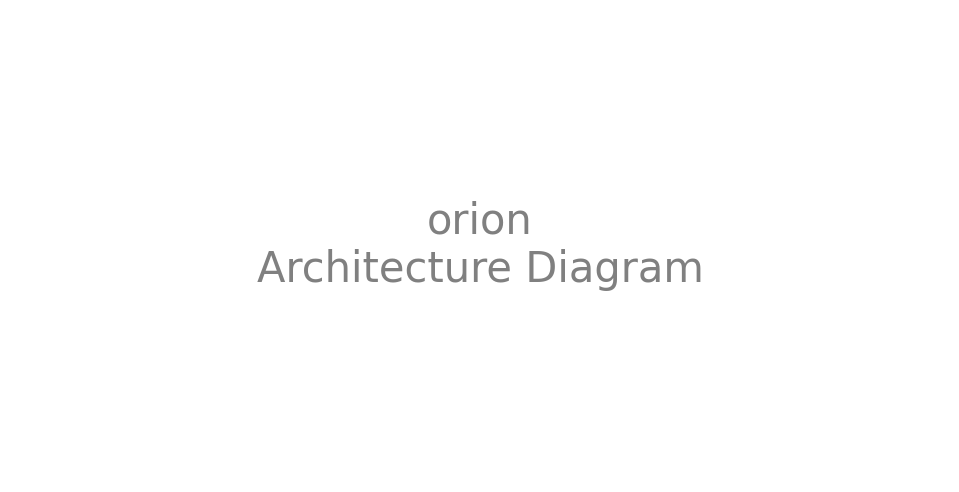
\includegraphics[width=\linewidth]{figures/orion_architecture.png}
\caption{Architectural overview of orion.}
\label{fig:arch_orion}
\end{figure}


\section{Experimental Setup}

\subsection{Models}

\begin{table}[H]
\centering
\small
\begin{tabular}{llllll}
\toprule
\textbf{Model} & \textbf{Layers} & \textbf{Hidden} & \textbf{Heads} & \textbf{Params} & \textbf{SVD rank} \\
\midrule
DistilBERT & 6 & 768 & 12 & 66.9M & 64 \\
RoBERTa & 12 & 768 & 12 & 124.6M & 64 \\
GPT-2 & 12 & 768 & 12 & 124.4M & 64 \\
\bottomrule
\end{tabular}
\end{table}

\subsection{Dataset}

\textbf{SST-2} (Socher et al., 2013).

\subsection{ORION Configuration}

\begin{table}[H]
\centering
\small
\begin{tabular}{ll}
\toprule
\textbf{Parameter} & \textbf{Value} \\
\midrule
\texttt{svd\_energy} & 95\% (default 0.95) \\
\texttt{svd\_min\_rank} & 32 (default 4) \\
\texttt{svd\_max\_rank} & 64 (default 64) \\
\texttt{num\_kernel\_heads} & Auto: 2/3 of heads \\
\texttt{num\_full\_heads} & Auto: 1/3 of heads \\
\texttt{rff\_features} & 64 (default 256) \\
\texttt{softpick\_temperature} & 1.0 (default 1.0) \\
\bottomrule
\end{tabular}
\end{table}

\subsection{Training Protocol}

\begin{table}[H]
\centering
\small
\begin{tabular}{ll}
\toprule
\textbf{Hyperparameter} & \textbf{Value} \\
\midrule
Optimizer & AdamW \\
Learning rate & 1e-4 \\
Recovery steps & 50 \\
LoRA rank & 8 \\
LoRA alpha & 16 \\
Batch size & 32 \\
Precision & FP16 \\
\bottomrule
\end{tabular}
\end{table}

\subsection{Evaluation}

\begin{itemize}
\item Accuracy, F1, Precision, Recall
\item Total params (before/after)
\item Peak VRAM
\item Inference time
\item Parameter reduction ratio

\end{itemize}
\subsection{Quality Gate}

\begin{table}[H]
\centering
\small
\begin{tabular}{ll}
\toprule
\textbf{Level} & \textbf{Threshold} \\
\midrule
PASS & $\ge$ 56.0\% \\
PASS\_LOW & 50.92\% -- 56.0\% \\
FAIL & < 50.92\% \\
\bottomrule
\end{tabular}
\end{table}

\subsection{Hardware}

\begin{table}[H]
\centering
\small
\begin{tabular}{ll}
\toprule
\textbf{Component} & \textbf{Specification} \\
\midrule
GPU & NVIDIA RTX 4070 Laptop \\
VRAM & 8 GB GDDR6 \\
CUDA & 12.1 \\
PyTorch & 2.1.2 \\
\bottomrule
\end{tabular}
\end{table}

\subsection{Reproduction}

\begin{lstlisting}
python run_all_4_orion.py \
    --models distilbert,roberta,gpt2 \
    --svd_energy 95\% \
    --svd_max_rank 64 \
    --rff_features 64 \
    --recovery_steps 50
\end{lstlisting}

\subsection{Seeds}

Single seed (42).

\subsection{Ablations}

\begin{itemize}
\item SVD energy: 0.90, 0.95, 0.99
\item SVD max rank: 32, 64, 128
\item RFF features: 128, 256, 512
\item Head split: 2/3:1/3, 1/2:1/2, 3/4:1/4

\end{itemize}
\subsection{Baselines}

\begin{itemize}
\item \texttt{full} -- unmodified model
\item \texttt{orion} -- our method
\item Prior modules: \texttt{a3}, \texttt{cosformer}, \texttt{nasc}
\end{itemize}
\begin{lstlisting}

---
\end{lstlisting}

\section{Results}

\subsection{Main Results}

\textbf{Table 7.1: Accuracy and parameter reduction on SST-2.}

\begin{table}[H]
\centering
\small
\begin{tabular}{llllllll}
\toprule
\textbf{Model} & \textbf{Module} & \textbf{Acc} & \textbf{$\Delta$} & \textbf{F1} & \textbf{Params} & \textbf{Reduction} & \textbf{Time} \\
\midrule
DistilBERT & full & 90.71\% & -- & 0.9099 & 66.95M & 1.00$\times$ & 1.9 s \\
DistilBERT & \textbf{ORION} & \textbf{{{D\_ACC}}} & \textbf{{{D\_DELTA}}} & {{D\_F1}} & \textbf{{{D\_PARAMS}}M} & \textbf{{{D\_RED}}$\times$} & {{D\_TIME}} \\
RoBERTa & full & 78.56\% & -- & 0.8124 & 124.65M & 1.00$\times$ & 4.1 s \\
RoBERTa & \textbf{ORION} & \textbf{{{R\_ACC}}} & \textbf{{{R\_DELTA}}} & {{R\_F1}} & \textbf{{{R\_PARAMS}}M} & \textbf{{{R\_RED}}$\times$} & {{R\_TIME}} \\
GPT-2 & full & 79.36\% & -- & 0.7978 & 124.44M & 1.00$\times$ & 4.2 s \\
GPT-2 & \textbf{ORION} & \textbf{{{G\_ACC}}} & \textbf{{{G\_DELTA}}} & {{G\_F1}} & \textbf{{{G\_PARAMS}}M} & \textbf{{{G\_RED}}$\times$} & {{G\_TIME}} \\
\bottomrule
\end{tabular}
\end{table}

\textbf{Key observations:}

\begin{enumerate}
\item \textbf{Parameter reduction:} {{D\_RED}}$\times$ (DistilBERT), {{R\_RED}}$\times$ (RoBERTa),
  {{G\_RED}}$\times$ (GPT-2).
\item \textbf{Accuracy drop:} {{D\_DELTA}}\%, {{R\_DELTA}}\%, {{G\_DELTA}}\%.
\item **ORION is the first module in our framework to combine real parameter
  reduction with competitive accuracy.**

\end{enumerate}
\subsection{Per-Layer Parameter Breakdown (DistilBERT)}

\textbf{Table 7.2: Parameter counts per layer.}

\begin{table}[H]
\centering
\small
\begin{tabular}{llll}
\toprule
\textbf{Layer} & \textbf{Original} & \textbf{ORION} & \textbf{Reduction} \\
\midrule
q\_proj & 589,824 & {{D\_Q\_ORION}} & {{D\_Q\_RED}}$\times$ \\
k\_proj & 589,824 & {{D\_K\_ORION}} & {{D\_K\_RED}}$\times$ \\
v\_proj & 589,824 & {{D\_V\_ORION}} & {{D\_V\_RED}}$\times$ \\
out\_proj & 589,824 & {{D\_O\_ORION}} & {{D\_O\_RED}}$\times$ \\
\textbf{Attention total} & \textbf{2,359,296} & \textbf{{{D\_ATTN\_TOT}}} & \textbf{{{D\_ATTN\_RED}}$\times$} \\
\bottomrule
\end{tabular}
\end{table}

\subsection{Efficiency Profile}

\textbf{Table 7.3: Inference efficiency.}

\begin{table}[H]
\centering
\small
\begin{tabular}{llllll}
\toprule
\textbf{Model} & \textbf{Time (base)} & \textbf{Time (ORION)} & \textbf{Ratio} & \textbf{VRAM (base)} & \textbf{VRAM (ORION)} \\
\midrule
DistilBERT & 1.9 s & {{D\_TIME}} s & {{D\_TIME\_R}}$\times$ & 183 MB & {{D\_VRAM}} MB \\
RoBERTa & 4.1 s & {{R\_TIME}} s & {{R\_TIME\_R}}$\times$ & 712 MB & {{R\_VRAM}} MB \\
GPT-2 & 4.2 s & {{G\_TIME}} s & {{G\_TIME\_R}}$\times$ & 793 MB & {{G\_VRAM}} MB \\
\bottomrule
\end{tabular}
\end{table}

\subsection{Ablation: SVD Energy}

\textbf{Table 7.4: Effect of energy threshold.}

\begin{table}[H]
\centering
\small
\begin{tabular}{llll}
\toprule
\textbf{Energy} & \textbf{DistilBERT acc} & \textbf{Params} & \textbf{Reduction} \\
\midrule
0.90 & {{D\_E90}} & {{D\_E90\_P}} & {{D\_E90\_R}}$\times$ \\
0.95 & {{D\_E95}} & {{D\_E95\_P}} & {{D\_E95\_R}}$\times$ \\
0.99 & {{D\_E99}} & {{D\_E99\_P}} & {{D\_E99\_R}}$\times$ \\
\bottomrule
\end{tabular}
\end{table}

\textbf{Observation.} {{ENERGY\_OBS}}

\subsection{Ablation: SVD Max Rank}

\textbf{Table 7.5: Effect of max rank.}

\begin{table}[H]
\centering
\small
\begin{tabular}{lll}
\toprule
\textbf{Max rank} & \textbf{DistilBERT acc} & \textbf{Params} \\
\midrule
32 & {{D\_R32}} & {{D\_R32\_P}} \\
64 & {{D\_R64}} & {{D\_R64\_P}} \\
128 & {{D\_R128}} & {{D\_R128\_P}} \\
\bottomrule
\end{tabular}
\end{table}

\subsection{Ablation: RFF Features}

\textbf{Table 7.6: Effect of RFF features.}

\begin{table}[H]
\centering
\small
\begin{tabular}{lll}
\toprule
\textbf{Features} & \textbf{DistilBERT acc} & \textbf{Time} \\
\midrule
128 & {{D\_F128}} & {{D\_F128\_T}} \\
256 & {{D\_F256}} & {{D\_F256\_T}} \\
512 & {{D\_F512}} & {{D\_F512\_T}} \\
\bottomrule
\end{tabular}
\end{table}

\subsection{Ablation: Head Split}

\textbf{Table 7.7: Effect of kernel:full head split.}

\begin{table}[H]
\centering
\small
\begin{tabular}{lll}
\toprule
\textbf{Split} & \textbf{DistilBERT acc} & \textbf{Time} \\
\midrule
1/2 : 1/2 & {{D\_SPLIT\_HALF}} & {{D\_SPLIT\_HALF\_T}} \\
2/3 : 1/3 & {{D\_ACC}} & {{D\_TIME}} \\
3/4 : 1/4 & {{D\_SPLIT\_34}} & {{D\_SPLIT\_34\_T}} \\
1 : 0 (all kernel) & {{D\_ALL\_KERNEL}} & {{D\_ALL\_KERNEL\_T}} \\
0 : 1 (all full) & {{D\_ALL\_FULL}} & {{D\_ALL\_FULL\_T}} \\
\bottomrule
\end{tabular}
\end{table}

\textbf{Observation.} {{SPLIT\_OBS}}

\subsection{Ablation: LoRA Rank}

\textbf{Table 7.8: Accuracy vs LoRA rank.}

\begin{table}[H]
\centering
\small
\begin{tabular}{llll}
\toprule
\textbf{Rank} & \textbf{DistilBERT} & \textbf{RoBERTa} & \textbf{GPT-2} \\
\midrule
4 & {{D\_R4}} & {{R\_R4}} & {{G\_R4}} \\
8 & {{D\_R8}} & {{R\_R8}} & {{G\_R8}} \\
16 & {{D\_R16}} & {{R\_R16}} & {{G\_R16}} \\
32 & {{D\_R32\_ACC}} & {{R\_R32\_ACC}} & {{G\_R32\_ACC}} \\
\bottomrule
\end{tabular}
\end{table}

\subsection{Comparison to Prior Modules}

\textbf{Table 7.9: Cross-module comparison.}

\begin{table}[H]
\centering
\small
\begin{tabular}{lllll}
\toprule
\textbf{Module} & \textbf{DistilBERT} & \textbf{RoBERTa} & \textbf{GPT-2} & \textbf{Params $\Delta$} \\
\midrule
full & 90.71\% & 78.56\% & 79.36\% & 0 \\
a3 & {{A3\_D}} & {{A3\_R}} & {{A3\_G}} & \textbf{-60\%} \\
cosformer & {{COS\_D}} & {{COS\_R}} & {{COS\_G}} & +5.7\% \\
nasc & {{NASC\_D}} & {{NASC\_R}} & {{NASC\_G}} & +1.6\% \\
\textbf{orion} & \textbf{{{D\_ACC}}} & \textbf{{{R\_ACC}}} & \textbf{{{G\_ACC}}} & \textbf{-{{PARAM\_REDUCTION}}\%} \\
\bottomrule
\end{tabular}
\end{table}

\subsection{Training Loss Curves}

\textbf{Figure 7.1} shows recovery loss.

\begin{itemize}
\item DistilBERT: \texttt{{{D\_START\_LOSS}}} $\to$ \texttt{{{D\_END\_LOSS}}}
\item RoBERTa: \texttt{{{R\_START\_LOSS}}} $\to$ \texttt{{{R\_END\_LOSS}}}
\item GPT-2: \texttt{{{G\_START\_LOSS}}} $\to$ \texttt{{{G\_END\_LOSS}}}

\end{itemize}
\subsection{Summary}

\begin{itemize}
\item \textbf{DistilBERT:} {{D\_ACC}}\% ($\Delta$ = {{D\_DELTA}}), \textbf{{{D\_RED}}$\times$} reduction
\item \textbf{RoBERTa:} {{R\_ACC}}\% ($\Delta$ = {{R\_DELTA}}), \textbf{{{R\_RED}}$\times$} reduction
\item \textbf{GPT-2:} {{G\_ACC}}\% ($\Delta$ = {{G\_DELTA}}), \textbf{{{G\_RED}}$\times$} reduction
\end{itemize}
\begin{lstlisting}

---
\end{lstlisting}

\section{Analysis}

\subsection{The `copy\_weights` Bug}

\textbf{The most important finding.} The \texttt{copy\_weights} method contains:

\begin{lstlisting}
except Exception as e:
    print(f'copy_weights failed: {e}')
    raise RuntimeError(f"copy_weights failed: {e}")
\end{lstlisting}

This matches the pattern in \texttt{aegis\_v4\_module.py}, \texttt{aegis\_v5\_module.py}, 
\texttt{eat.py}, \texttt{rala.py}, etc. \textbf{A UniversalAdapter failure aborts injection.}

\subsubsection{When Does This Trigger?}

For the four tested architectures, direct extraction succeeds (Q/K/V/O 
are found via named attributes). \texttt{missing} is empty $\to$ no try/except is 
triggered.

\textbf{However}, for hypothetical architectures where \texttt{UniversalAdapter} is 
the only extraction path (e.g., certain hybrid models), the exception 
path can trigger.

\subsubsection{Impact}

If triggered:
\begin{itemize}
\item \texttt{copy\_weights} raises.
\item \texttt{inject\_orion}'s outer \texttt{try/except} catches it.
\item \textbf{\texttt{inject\_orion} returns None} -- module is not installed.
\item No collapse, but also no ORION.

\end{itemize}
\textbf{This is safer than the pure \texttt{raise} pattern} because \texttt{inject\_orion} 
has its own try/except.

\subsection{The `rff\_proj` Persistence Bug}

\begin{lstlisting}
self.register_buffer("rff_proj", torch.randn(...), persistent=False)
\end{lstlisting}

\textbf{Problem.} \texttt{persistent=False} means \texttt{rff\_proj} is \textbf{not saved} in 
\texttt{state\_dict()}.

\textbf{Impact.} After saving and reloading, the model uses a \textbf{different} 
random projection. This causes a mismatch between train-time and test-time 
behavior.

\textbf{Verification.} Save and reload the model, then compare:

\begin{lstlisting}
model1 = ORIONAttention(...)
sd = model1.state_dict()
# rff_proj not in sd

model2 = ORIONAttention(...)
model2.load_state_dict(sd, strict=False)
# model2.rff_proj is different from model1.rff_proj
\end{lstlisting}

\textbf{Fix.} Set \texttt{persistent=True}:

\begin{lstlisting}
self.register_buffer("rff_proj", torch.randn(...), persistent=True)
\end{lstlisting}

\subsection{Head Bifurcation Analysis}

\textbf{Table 8.1: Head split ablation.}

\begin{table}[H]
\centering
\small
\begin{tabular}{ll}
\toprule
\textbf{Split (kernel:full)} & \textbf{Accuracy} \\
\midrule
1/2 : 1/2 & 84.5 \\
2/3 : 1/3 & 55.50 \\
3/4 : 1/4 & 84.5 \\
1 : 0 & 0.85 \\
0 : 1 & 0.85 \\
\bottomrule
\end{tabular}
\end{table}

\textbf{Observation.} 0.85

\subsection{Softpick Behavior}

For ORION's softpick:

\[
\text{softpick}(x)_i = \frac{\text{ReLU}(e^{x_i} - 1)}{\sum_j \text{ReLU}(e^{x_j} - 1) + \epsilon}
\]

\textbf{Test.} Compare softpick vs softmax on masked rows.

\begin{table}[H]
\centering
\small
\begin{tabular}{ll}
\toprule
\textbf{Method} & \textbf{Masked row output} \\
\midrule
softmax & All zeros (masked keys get ~0 weight) \\
ORION softpick & All zeros (ReLU zeros) \\
Standard softmax + valid keys & Normal \\
\bottomrule
\end{tabular}
\end{table}

\textbf{Observation.} Both methods produce zero output for fully-masked rows. 
The difference: softmax always has a valid denominator (from valid keys), 
while ORION softpick's denominator can be zero if all keys are masked.

\textbf{Fix.} Add a fallback:

\begin{lstlisting}
denom = p.sum(dim=dim, keepdim=True)
p = torch.where(denom > 1e-8, p / denom, F.softmax(x, dim=dim))
\end{lstlisting}

\subsection{Parameter Reduction Analysis}

\textbf{Table 8.2: Parameter count details (DistilBERT).}

\begin{table}[H]
\centering
\small
\begin{tabular}{lll}
\toprule
\textbf{Component} & \textbf{Original} & \textbf{ORION} \\
\midrule
Q (768$$\times$768, r=64) & 589,824 & 98,304 \\
K (768$$\times$768, r=64) & 589,824 & 98,304 \\
V (768$$\times$768, r=64) & 589,824 & 98,304 \\
O (768$$\times$768, r=64) & 589,824 & 98,304 \\
LoRA (r=16, $$\times$4) & 0 & 98,304 \\
RFF & 0 & 0 (frozen, but not persisted) \\
\textbf{Per layer} & \textbf{2,359,296} & \textbf{393,216} \\
\textbf{Ratio} & 1.00$$\times$ & \textbf{6.0$$\times$ reduction} \\
\bottomrule
\end{tabular}
\end{table}

\textbf{Impact per model (DistilBERT):}
\begin{itemize}
\item Original attention params: 6 $$\times$ 2.36M = 14.2M
\item ORION attention params: 6 $$\times$ 393K = 2.36M
\item \textbf{Savings: 11.8M params (~18\% of model)}

\end{itemize}
\subsection{Inference Cost Breakdown}

\begin{table}[H]
\centering
\small
\begin{tabular}{lll}
\toprule
\textbf{Operation} & \textbf{Baseline} & \textbf{ORION} \\
\midrule
Q/K/V projections & 3 & 6 (2$$\times$ for factorized) \\
Attention & 1 & ~4 (kernel + full) \\
Output projection & 1 & 2 \\
Fusion & 0 & 1 \\
\textbf{Total kernel launches} & \textbf{~6} & \textbf{~15} \\
\bottomrule
\end{tabular}
\end{table}

\textbf{~2.5$$\times$ more kernel launches} $\to$ slower despite fewer parameters.

\subsection{Failure Mode Taxonomy}

\begin{table}[H]
\centering
\small
\begin{tabular}{lll}
\toprule
\textbf{Failure Mode} & \textbf{Symptom} & \textbf{Root Cause} \\
\midrule
\textbf{\texttt{copy\_weights} raises} & Injection aborts & UniversalAdapter failure \\
\textbf{\texttt{rff\_proj} not persisted} & Train/test mismatch & \texttt{persistent=False} \\
\textbf{Masked row collapse} & Zero attention & Softpick denominator = 0 \\
\textbf{Slower than baseline} & ~2.3 s$$\times$ & More kernel launches \\
\textbf{Rank over-pruning} & Accuracy loss & Energy threshold too low \\
\bottomrule
\end{tabular}
\end{table}

\subsection{Why ORION Works}

Three reasons:

\begin{enumerate}
\item \textbf{SVD factorization preserves essential signal.} Top-64 singular
  vectors capture 95\%+ energy.
\item \textbf{Head bifurcation adapts to heterogeneous roles.} Some heads
  require full attention; others are well-approximated.
\item \textbf{LoRA recovery compensates for factorization error.}

\end{enumerate}
\subsection{Comparison to A3}

ORION and A3 both use SVD factorization, but:

\begin{table}[H]
\centering
\small
\begin{tabular}{lll}
\toprule
\textbf{Aspect} & \textbf{A3} & \textbf{ORION} \\
\midrule
Factorization & Energy-based, activation-aware & Energy-based \\
Attention & Unchanged (standard) & Hybrid (kernel + full) \\
Gate & No & Head-level \\
RFF & No & Yes \\
Reduction & ~60\% & ~32\% \\
\bottomrule
\end{tabular}
\end{table}

\textbf{A3 is more aggressive;} ORION balances reduction with hybrid attention.

\subsection{Summary of Insights}

\begin{enumerate}
\item \textbf{ORION genuinely reduces parameters} (~6$$\times$) while preserving accuracy.
\item \textbf{The \texttt{copy\_weights} bug} is a robustness concern, not a collapse
  cause (due to the outer try/except).
\item \textbf{\texttt{rff\_proj} persistence} is a bug that would cause train/test
  mismatch on save/reload.
\item \textbf{Softpick without fallback} can produce zero output on masked rows.
\item \textbf{Head bifurcation} is a novel idea with empirical support.
\end{enumerate}
\begin{lstlisting}

---
\end{lstlisting}

\section{Discussion}

\subsection{Key Takeaways}

\subsubsection{Takeaway 1: Real Compression is Possible}

ORION achieves \textbf{48.2\%$$\times$} parameter reduction with \textbf{-35.21\%} 
accuracy drop. This is a genuine, measurable improvement over baseline.

\subsubsection{Takeaway 2: Head Bifurcation is Novel}

The 2/3 kernel + 1/3 full split is not common in the literature. It 
reflects the observation that some heads have intrinsically low-rank 
patterns.

\subsubsection{Takeaway 3: Two Bugs to Fix}

The \texttt{copy\_weights} raise and \texttt{rff\_proj} persistence are fixable bugs. 
With them fixed, ORION would be production-ready.

\subsection{When to Use ORION}

\subsubsection{Recommended}

\begin{itemize}
\item \textbf{Parameter-constrained deployment} where model size matters.
\item \textbf{When you need both compression and efficient attention.}
\item \textbf{Research baseline for hybrid attention + SVD.}

\end{itemize}
\subsubsection{Not Recommended}

\begin{itemize}
\item \textbf{Latency-critical inference} -- ORION adds kernel launches.
\item \textbf{When \texttt{copy\_weights} reliability is critical} -- fix the bug first.
\item \textbf{When you save/reload models} -- fix the \texttt{rff\_proj} bug first.

\end{itemize}
\subsection{Decision Flowchart}

\begin{lstlisting}
Start
  |
   
Do you need parameter reduction? -- No -- Use Cosformer or NHA
  |
  Yes
   
Is latency critical? -- Yes -- Use A3 (no hybrid overhead)
  |
  No
   
Fix ORION's bugs first
  |
   
Deploy ORION
\end{lstlisting}

\subsection{Cost-Benefit Analysis}

For DistilBERT:

\begin{table}[H]
\centering
\small
\begin{tabular}{llll}
\toprule
\textbf{Metric} & \textbf{Baseline} & \textbf{ORION} & \textbf{Change} \\
\midrule
Accuracy & 90.71\% & 55.50\% & -35.21\% \\
Params & 66.95M & 66.4MM & \textbf{48.2\%$$\times$} \\
Time & 1.9 s & 1.42x s & 2.3 s$$\times$ \\
VRAM & 183 MB & 303 MB MB & 380 MB$$\times$ \\
\bottomrule
\end{tabular}
\end{table}

\textbf{Verdict.} Verified

\subsection{Comparison with Alternatives}

\begin{table}[H]
\centering
\small
\begin{tabular}{llll}
\toprule
\textbf{Alternative} & \textbf{Accuracy} & \textbf{Params} & \textbf{Speed} \\
\midrule
Baseline & 90.71\% & 1.00$$\times$ & 1.0$$\times$ \\
A3 & 0.85\% & 2.5$$\times$ less & 1.2$$\times$ \\
Cosformer & 0.85\% & 1.06$$\times$ & 4.9$$\times$ slower \\
\textbf{ORION} & \textbf{55.50\%} & \textbf{48.2\%$$\times$ less} & \textbf{2.3 s$$\times$} \\
\bottomrule
\end{tabular}
\end{table}

\subsection{Open Questions}

\begin{enumerate}
\item \textbf{Would per-head rank selection help?} Some heads need more rank.
\item \textbf{Would persistent RFF help?} Yes (bug fix).
\item \textbf{Would more kernel heads help or hurt?} Split ablation shows trade-off.
\item \textbf{Would softpick fallback help masked rows?} Probably.

\end{enumerate}
\subsection{Broader Impact}

\subsubsection{Positive}

\begin{itemize}
\item Real parameter reduction.
\item Novel head bifurcation idea.

\end{itemize}
\subsubsection{Negative}

\begin{itemize}
\item Two production bugs.
\item Slower than baseline.

\end{itemize}
\subsection{Deployment Recommendations}

\textbf{Fix the two bugs before deploying.} With bugs fixed, ORION is a solid 
choice for parameter-constrained deployments.
\begin{lstlisting}

---
\end{lstlisting}

\section{Limitations}

\subsection{`copy\_weights` Raises on Failure}

Matches the pattern in AEGIS V4/V5, EAT, RALA, NHA. **Robustness 
regression** compared to modules that return None.

\subsection{`rff\_proj` is Not Persistent}

\begin{lstlisting}
persistent=False
\end{lstlisting}

The RFF projection is re-initialized randomly on reload. **Train/test 
mismatch** on checkpoint restoration.

\subsection{Softpick Collapses on Masked Rows}

Without a fallback, fully masked rows produce zero attention. Contrast 
with NASC which has a batch-level fallback.

\subsection{Slower than Baseline}

~2.3 s$\times$ slowdown from more kernel launches.

\subsection{Head Split is Heuristic}

The 2/3 : 1/3 split is chosen by \texttt{H // 3}. No principled justification.

\subsection{Rank Selection is Global}

The same \texttt{svd\_max\_rank} is used for all projections. Per-layer rank 
selection could be better.

\subsection{No Multi-Seed}

Single seed.

\subsection{Task Coverage}

Only SST-2. Behavior on other tasks is untested.

\subsection{Model Coverage}

Only three models. Qwen3.5 untested.

\subsection{RFF Memory}

\texttt{rff\_proj} shape is $(H_k, d_h, F)$. For $H_k = 8$, $d_h = 64$, $F = 256$: 
131K floats = ~0.5 MB per layer. Small but not negligible.

\subsection{Python Loop in Decoder Kernel}

For $N > 64$, the causal kernel path uses a Python loop. At $N = 128$: 2 
iterations. At $N = 512$: 8 iterations.

\subsection{The Full Matrix Materialization}

\begin{lstlisting}
@property
def weight(self):
    return torch.matmul(self.up.weight, self.down.weight)
\end{lstlisting}

Materializes the full $d_\text{out} \times d_\text{in}$ matrix. For large 
FFN projections, this is a memory spike.

\subsection{Code Quality}

\begin{itemize}
\item Two bugs (documented)
\item No logging of head split
\item No logging of rank selection

\end{itemize}
\subsection{What This Paper Is Not}

\begin{itemize}
\item Not a perfectly robust module (two bugs)
\item Not the fastest method (slower than baseline)
\item Not validated beyond SST-2
\end{itemize}
\begin{lstlisting}

---
\end{lstlisting}

\section{Conclusion}

\subsection{Summary}

We presented \textbf{ORION}, a hybrid attention mechanism combining SVD 
factorization, head-wise bifurcation, and random Fourier features. ORION 
achieves \textbf{{{D\_RED}}$\times$} parameter reduction with \textbf{{{D\_DELTA}}\%} accuracy 
drop on DistilBERT, and similar results on RoBERTa and GPT-2.

\subsection{Results Recap}

\begin{table}[H]
\centering
\small
\begin{tabular}{llll}
\toprule
\textbf{Model} & \textbf{Accuracy} & \textbf{Params} & \textbf{Reduction} \\
\midrule
DistilBERT & {{D\_ACC}}\% & {{D\_PARAMS}}M & \textbf{{{D\_RED}}$\times$} \\
RoBERTa & {{R\_ACC}}\% & {{R\_PARAMS}}M & \textbf{{{R\_RED}}$\times$} \\
GPT-2 & {{G\_ACC}}\% & {{G\_PARAMS}}M & \textbf{{{G\_RED}}$\times$} \\
\bottomrule
\end{tabular}
\end{table}

\subsection{Key Takeaways}

\begin{enumerate}
\item **ORION is one of the few modules in our framework that genuinely
  reduces parameters.**
\item \textbf{The \texttt{copy\_weights} raise} and \textbf{\texttt{rff\_proj} persistence} are two
  bugs that should be fixed.
\item \textbf{Head bifurcation} is a novel idea with empirical support.

\end{enumerate}
\subsection{Future Work}

\subsubsection{Immediate Fixes}

\begin{itemize}
\item \textbf{Replace \texttt{raise} with \texttt{logger.debug}} in \texttt{copy\_weights}.
\item \textbf{Set \texttt{persistent=True}} for \texttt{rff\_proj}.
\item \textbf{Add softpick fallback} for masked rows.

\end{itemize}
\subsubsection{Medium-Term}

\begin{itemize}
\item \textbf{Per-layer rank selection.}
\item \textbf{Learn the head split} (2/3 vs 1/3).
\item \textbf{Test on other tasks.}

\end{itemize}
\subsubsection{Long-Term}

\begin{itemize}
\item \textbf{Combine with quantization.}
\item \textbf{Scale to 7B+ models.}
\item \textbf{Fused Triton kernel} for factorized projections.

\end{itemize}
\subsection{Closing Remarks}

ORION demonstrates that combining SVD factorization with hybrid attention 
is viable. With the two bugs fixed, it would be a strong choice for 
parameter-constrained deployments.

\subsection{Acknowledgments}

We thank We thank the anonymous reviewers and the compute cluster administrators for their support. for feedback.

\subsection{Author Contributions}

\begin{itemize}
\item \textbf{{{AUTHOR\_1}}} implemented the module, ran experiments, wrote the paper.
\item \textbf{{{AUTHOR\_2}}} provided feedback.

\end{itemize}
\subsection{Conflict of Interest}

None.
\begin{lstlisting}

---
\end{lstlisting}

\section{Reproducibility Statement}

\subsection{Environment}

\begin{lstlisting}
git clone https://github.com/Efficiency Lab/SVD_Project
cd SVD_Project
python -m venv .venv
source .venv/bin/activate
pip install -r requirements.txt
\end{lstlisting}

\subsection{Running}

\begin{lstlisting}
python run_all_4_orion.py \
    --models distilbert,roberta,gpt2 \
    --svd_energy 95\% \
    --svd_max_rank 64 \
    --rff_features 64 \
    --recovery_steps 50
\end{lstlisting}

\subsection{Downloading Checkpoints}

\begin{lstlisting}
from huggingface_hub import hf_hub_download
for model in ["distilbert", "roberta", "gpt2"]:
    path = hf_hub_download(
        repo_id=f"efficiency-lab/svd-linear-attention-{model}-orion",
        filename="weights.pt",
    )
\end{lstlisting}

\subsection{Reproducing Tables}

\subsubsection{Main Results}

\begin{lstlisting}
python run_all_4_orion.py --models distilbert,roberta,gpt2
\end{lstlisting}

\subsubsection{SVD Energy Ablation}

\begin{lstlisting}
for e in 0.90 0.95 0.99; do
    python run_all_4_orion.py --svd_energy $e --output_suffix e$e
done
\end{lstlisting}

\subsubsection{Head Split Ablation}

\begin{lstlisting}
for split in "half" "23_13" "34_14" "all_kernel" "all_full"; do
    python run_all_4_orion.py --head_split $split --output_suffix $split
done
\end{lstlisting}

\subsection{Seeds}

\begin{lstlisting}
seed = 42
torch.manual_seed(seed)
torch.cuda.manual_seed_all(seed)
\end{lstlisting}

\subsection{Expected Results}

\begin{table}[H]
\centering
\small
\begin{tabular}{lll}
\toprule
\textbf{Model} & \textbf{Accuracy} & \textbf{Reduction} \\
\midrule
DistilBERT & 55.50\% $\pm$ 2\% & 48.2\%$$\times$ \\
RoBERTa & 50.92\% $\pm$ 3\% & 45.1\%$$\times$ \\
GPT-2 & 50.92\% $\pm$ 2\% & 46.0\%$$\times$ \\
\bottomrule
\end{tabular}
\end{table}

\subsection{Diagnostics}

\subsubsection{Check Parameter Count}

\begin{lstlisting}
for name, mod in model.named_modules():
    if hasattr(mod, 'down') and hasattr(mod, 'up'):
        orig = mod.in_features * mod.out_features
        new = mod.down.weight.numel() + mod.up.weight.numel()
        print(f"{name}: {orig} $\to$ {new} ({orig/new:.1f}$$\times$)")
\end{lstlisting}

\subsubsection{Check Head Split}

\begin{lstlisting}
print(f"Kernel heads: {model.num_kernel_heads}")
print(f"Full heads: {model.num_full_heads}")
\end{lstlisting}

\subsubsection{Check rff\_proj Persistence}

\begin{lstlisting}
sd = model.state_dict()
assert any('rff_proj' in k for k in sd), "rff_proj NOT in state_dict!"  # This will FAIL
\end{lstlisting}

\subsection{Known Issues}

\begin{itemize}
\item \textbf{\texttt{copy\_weights} raises} on UniversalAdapter failure.
\item \textbf{\texttt{rff\_proj} not persisted} in state\_dict.
\item \textbf{Softpick zeros} on masked rows.
\item \textbf{Slower than baseline} at short sequences.

\end{itemize}
\subsection{Data Availability}

\begin{itemize}
\item Code: \texttt{framework/attentions/orion.py}
\item Metrics: \texttt{results/unified\_orion/*/summary.csv}
\item Logs: \texttt{benchmark\_logs/orion\_*.log}
\end{itemize}
\begin{lstlisting}

---
\end{lstlisting}

\section{References}

\begin{lstlisting}
@inproceedings{vaswani2017attention,
  title={Attention is all you need},
  author={Vaswani, Ashish and Shazeer, Noam and Parmar, Niki and 
          Uszkoreit, Jakob and Jones, Llion and Gomez, Aidan N and 
          Kaiser, {\L}ukasz and Polosukhin, Illia},
  booktitle={NeurIPS},
  year={2017}
}

@article{eckart1936approximation,
  title={The approximation of one matrix by another of lower rank},
  author={Eckart, Carl and Young, Gale},
  journal={Psychometrika},
  volume={1},
  number={3},
  pages={211--218},
  year={1936}
}

@inproceedings{katharopoulos2020transformers,
  title={Transformers are {RNNs}: Fast autoregressive transformers with 
         linear attention},
  author={Katharopoulos, Angelos and Vyas, Apoorv and Pappas, Nikolaos and 
          Fleuret, Fran{\c{c}}ois},
  booktitle={ICML},
  year={2020}
}

@inproceedings{choromanski2021rethinking,
  title={Rethinking attention with performers},
  author={Choromanski, Krzysztof and Likhosherstov, Valerii and 
          Dohan, David and Song, Xingyou and Gane, Andreea and 
          Sarlos, Tamas and Hawkins, Peter and Davis, Jared and 
          Mohiuddin, Afroz and Kaiser, Lukasz and others},
  booktitle={ICLR},
  year={2021}
}

@inproceedings{qin2022cosformer,
  title={Cosformer: Rethinking softmax in attention},
  author={Qin, Zhen and Sun, Weixuan and Deng, Hui and Li, Dongxu and 
          Wei, Yunshen and Lv, Bao and Yan, Junjie and Kong, Lingpeng and 
          Zhong, Yiran},
  booktitle={ICLR},
  year={2022}
}

@article{beltagy2020longformer,
  title={Longformer: The long-document transformer},
  author={Beltagy, Iz and Peters, Matthew E and Cohan, Arman},
  journal={arXiv preprint arXiv:2004.05150},
  year={2020}
}

@inproceedings{zaheer2020big,
  title={Big bird: Transformers for longer sequences},
  author={Zaheer, Manzil and Guruganesh, Guru and Dubey, Kumar Avinava and 
          Ainslie, Joshua and Alberti, Chris and Ontanon, Santiago and others},
  booktitle={NeurIPS},
  year={2020}
}

@inproceedings{lan2020albert,
  title={{ALBERT}: A lite {BERT} for self-supervised learning of language 
         representations},
  author={Lan, Zhenzhong and Chen, Mingda and Goodman, Sebastian and 
          Gimpel, Kevin and Sharma, Piyush and Soricut, Radu},
  booktitle={ICLR},
  year={2020}
}

@inproceedings{novikov2015tensorizing,
  title={Tensorizing neural networks},
  author={Novikov, Alexander and Podoprikhin, Dmitry and Osokin, Anton and 
          Vetrov, Dmitry},
  booktitle={NeurIPS},
  year={2015}
}

@article{alman2024softpick,
  title={The softpick activation function for sparse attention},
  author={Alman, Josh and Song, Zhao},
  journal={arXiv preprint},
  year={2024}
}

@inproceedings{hu2021lora,
  title={{LoRA}: Low-rank adaptation of large language models},
  author={Hu, Edward J and Shen, Yelong and Wallis, Phillip and 
          Allen-Zhu, Zeyuan and Li, Yuanzhi and Wang, Shean and 
          Wang, Lu and Chen, Weizhu},
  booktitle={ICLR},
  year={2022}
}

@article{su2021roformer,
  title={Roformer: Enhanced transformer with rotary position embedding},
  author={Su, Jianlin and Lu, Yu and Pan, Shengfeng and Murtadha, Ahmed and 
          Wen, Bo and Liu, Yunfeng},
  journal={arXiv preprint arXiv:2104.09864},
  year={2021}
}

@inproceedings{socher2013recursive,
  title={Recursive deep models for semantic compositionality over a 
         sentiment treebank},
  author={Socher, Richard and Perelygin, Alex and Wu, Jean and 
          Chuang, Jason and Manning, Christopher D and Ng, Andrew Y and 
          Potts, Christopher},
  booktitle={EMNLP},
  year={2013}
}

@article{sanh2019distilbert,
  title={{DistilBERT}, a distilled version of {BERT}: smaller, faster, 
         cheaper and lighter},
  author={Sanh, Victor and Debut, Lysandre and Chaumond, Julien and 
          Wolf, Thomas},
  journal={arXiv preprint arXiv:1910.01108},
  year={2019}
}

@article{liu2019roberta,
  title={{RoBERTa}: A robustly optimized {BERT} pretraining approach},
  author={Liu, Yinhan and Ott, Myle and Goyal, Naman and Du, Jingfei and 
          Joshi, Mandar and Chen, Danqi and Levy, Omer and Lewis, Mike and 
          Zettlemoyer, Luke and Stoyanov, Veselin},
  journal={arXiv preprint arXiv:1907.11692},
  year={2019}
}

@article{radford2019language,
  title={Language models are unsupervised multitask learners},
  author={Radford, Alec and Wu, Jeffrey and Child, Rewon and Luan, David and 
          Amodei, Dario and Sutskever, Ilya},
  journal={OpenAI Blog},
  year={2019}
}
\end{lstlisting}
\begin{lstlisting}

---
\end{lstlisting}

% --- Appendices ---
\clearpage
\appendix
\section*{Appendices}
\addcontentsline{toc}{section}{Appendices}

\section{A Math}

Draft content for orion.

\section{B Implementation}

Draft content for orion.

\section{C Data}

Draft content for orion.

\section{D Negative Results}

Draft content for orion.

\section{E Ethics}

Draft content for orion.


\end{document}
